\documentclass[12pt]{article}
\usepackage[utf8]{inputenc}
\usepackage{mathtools}
\usepackage{amssymb}
\usepackage{amsmath}
\usepackage{amsthm}
\usepackage{array}
\usepackage{setspace}
\usepackage{parskip}
\usepackage{listings}
\title{Datenbanksysteme\\
			 Projekt Iteration 1: Modellierung}
\author{Adrian Gruszczynski\\ 
			Florian Brinkmeyer \\ %Informatik Lehramt
			Pit Ronk\\ %MAthe Bachelor
			Remi Toudic\\ %Mathe Master
		Tutor: Christian Hofmann\\
		Tutorium: Donnerstag 12-14}

\begin{document}
\maketitle
\section*{Aufgabe 1: Projektdokumentation}
Das Team in der alphabetischen Reihenfolge:
\begin{itemize}
\item Adrian Gruszczynski (Informatik Bachelor)
\item Florian Brinkmeyer (Informatik Lehramt)
\item Pit Ronk (Mathematik Bachelor)
\item Remi Toudic (Mathematik Master)
\end{itemize}


Projektziel 


Das Ziel des Projektes, ist die Entstehung einer Web Anwendung. Sie soll dabei Daten aus dem Datensatz \textit{american-election} in geeigneter Form, visuell darstellen sowie das Abfragen von Informationen ermöglichen. 

Das sekundäre Ziel ist dabei, das Auseinandersetzen mit relationale Datenbanken und deren Anwendung. 


Des Weiteren ist der Weg ebenso ein Ziel, welcher sich aus folgenden Punkten zusammen setzt. 

Phase 1: 
Hierbei liegt der Fokus auf der Festlegung der zu implementierenden Features sowie das Entwerfen des Konzeptes für das Datenmodell. 

Phase 2: 
Erstellung des Datenbankschemas sowie die Aufbereitung und das Pflegen der Daten. Des Weiteren folgt Einbindung in den Webserver.

Phase 3:
Bestimmung der Datenabhängigkeit sowie dessen visuelle Darstellung. 


\section*{Aufgabe 2: Explorative Datenanalyse}
\subsection*{Die einfache Analyse}
\subsection*{Die einfache Analyse}
Der Datensatz \textit{american-election-tweets.xlsx} besteht aus 6127 Einträgen und erfasst Tweets von Hillary Clinton und Donald Trump, sowie die Metadaten aus der Zeiten des Präsidentenwahl 2016 in Amerika.

Der Datensatz wird durch folgende Attribute charakterisiert:
\begin{itemize}
\item \textit{handle} : beschreibt den username des Tweet Authors
\item\textit{text} : speichert den textlichen Inhalt des Tweets
\item\textit{is\_reetwet} : sagt aus ob der jeweilige Tweet retweeted wurde. Kann nur boolean Werte annehmen
\item\textit{original\_author} : beschreibt den ursprünglichen Author des Tweets in falle eines retweets
\item\textit{time:} speichert den Zeitstempel jedes Tweets
\item\textit{in\_reply\_to\_screen\_name} : falls der Tweet ein reply ist speichert der Parameter den ursprünglichen Author
\item\textit{is\_quote\_status} : besagt ob der Tweet ein Zitat eines anderes Tweets ist. Kann nur boolean Werte annehmen
\item\textit{retweet\_count}: speichert wie viel Mal der jeweilige Tweet repostet/retweeted wurde
\item\textit{favorite\_count}: speichert wie viel Mal der jeweilige Tweet geliked wurde
\item\textit{source\_url}: beschreibt die Quelle des Tweets
\end{itemize}

\subsection*{Die explorative Analyse}
Der Datensatz beinhaltet Informationen über Tweets im Zeit des 01.05. bis 28.09.2016. Die Thematik behandelt die Präsidentenwahl in Amerika. Es gibt insgesamt 6126 Einträge von denen ca. 50.3\% von Hillary Clinton und 49.7\% von Donald Trump erstellt wurden.

 Die Tweets von Hillary Clinton wurden insgesamt 9346511 Mal retweeted und 21026005 Mal als Favorit markiert. Die Tweets von Donald Trump wurden 17668486 Male retweeted und 50778572 Male als Favorit gekennzeichnet. 
 
Obwohl es im dem Datensatz etwas mehr Tweets von Hillary Clinton gibt, wurden die Tweets von Donald Trump fast doppelt oft geliked und retweeted.  
Die Anzahl der Retweets von Donald Trump macht somit 65\% der gesamten Retweets und 70\% der ganzen likes aus dem gegebenen Datensatz aus.

 Ein durchschnittlicher Tweet von Trump wurde 16.665 Male retweeted und 5.798 Male als favorite markiert. 
Ein durchschnittlicher Tweet von Clinton wurde 3.035 Male retweeted und 6.828 Male geliked.

\subsection*{Zusammenhänge der Daten}


Die Korrelationsmatrix der wichtigsten Parameter:

\centerline{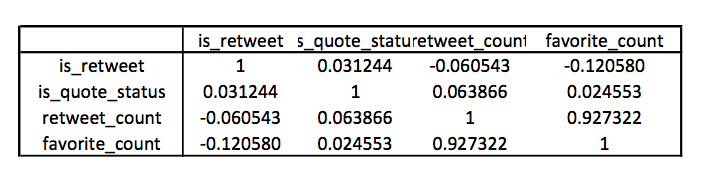
\includegraphics[scale=0.5]{img/marix.png} }

Die Anzahl der jeweiligen Tweets von Clinton und Trump werden graphisch wie folgt dargestellt:

\centerline{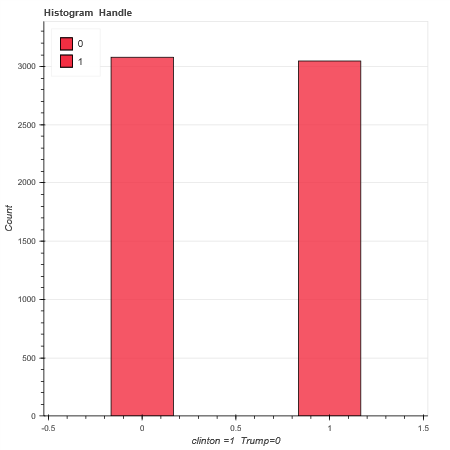
\includegraphics[scale=0.6]{img/histo_X.png} }


\centerline{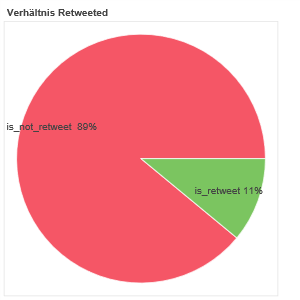
\includegraphics[scale=0.8]{img/pie_XX.png}}




\section*{Aufgabe 3: ER-Modellierung}
\centerline{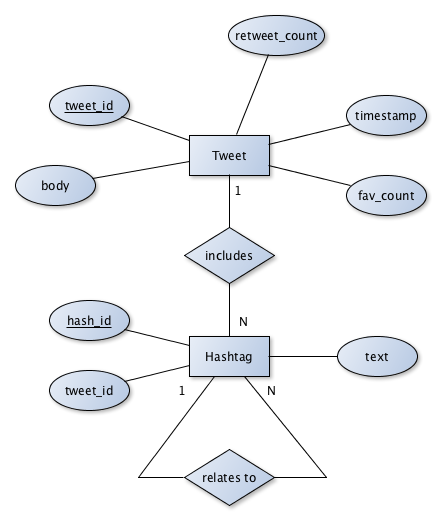
\includegraphics[scale=0.6]{img/img3.png} }
Das ER-Modell besteht aus 2 Entitätstypen, die die Datensätze aus jeweils gegebenen Attributen enthalten.
Der Entitätstyp 'Tweet' verfügt über folgende Attribute:
\begin{itemize}
\item \textit{tweet\_id}  ist ein Primärschlüssel der die Entitäten innerhalb des Entitätstyps eindeutig identifitzieren lässt.
\item \textit{body}: speichert den Inhalt jedes Tweets
\item \textit{fav\_count}: speichert die Anzahl der Likes für jede Instanz und lässt somit die Popularität eines Tweets abschätzen
\item \textit{retweet\_count}: speichert die Anzahl der Retweets für jede Instanz, kann als Kriterium sowohl für Popularität als auch  Wichtigkeit eines Tweets benutzt werden
\item \textit{timestamp}: speichert den timestamp (Zeitstempel) von jedem Tweet und kann im späteren Stadium dazu dienen, die Entwicklung von Hashtags über die Zeit zu analysieren
\end{itemize}

Der Entitätstyp Hashtag kapselt folgende Attributen:
\begin{itemize}
\item \textit{hash\_id}: ist ein Primärschlüssel der die Entitäten innerhalb des Entitätstyps eindeutig identifizieren lässt
\item \textit{tweet\_id}: ist ein Fremdschlüssel der jeder Hashtag Instanz den dazugehörigen Tweet zuordnen lässt
\item \textit{text}: speichert den Inhalt von jedem Hashtag
\end{itemize}

Jede Tweet Instanz kann, muss aber nicht, einen oder mehrere Hashtag Instanzen beinhalten. Jeder Hashtag Instanz wird anhand des Fremdschlüssels genau eine Tweet Entität zugeordnet.

Die Relation \textit{includes} ermöglicht dementsprechend für jeden Hashtags das dazugehörige Tweet zu zuordnen, und auch im späteren Stadium Zugriff auf die Attribute der beiden Entitäten.

Jede Hashtag Entität kann, muss aber nicht, mit einem oder mehreren Hashtags Entitäten in Relation stehen. Wenn zwei oder mehr Hashtags die selbe \textit{tweet\_id} zugeordnet wird bedeutet das, dass sie in Relation zueinander stehen, und tauchen zusammen in einem Tweet auf.

Die Relation \textit{relates\_to} erlaubt die Bestimmung des paarweisen Auftretens mehrerer Hashtags in einem Tweet.

Das obere ER-Model sowohl als auch das untere relationale Model, beinhalten nur ausgewählte Attribute aus dem gegebenen Datensatz.
Da die restlichen Attribute wie \textit{is\_retweet}, \textit{is\_quote\_status} usw. für die Anwendung unrelevant zu sein scheinen, haben wir uns entschieden diese vorerst zu ignorieren.

\newpage

\section*{Aufgabe 4: Relationales Modell}
$TWEET \{[tweet\_id:INT\, PRIMARY\, KEY, fav\_count:INT, timestamp:DATETIME(YYYY-MM-DDThh:mm:ss), retweet\_count:INT,$ 
$ body:TEXT(200)] \}$

$HASHTAG\{[hash\_id:INT\, PRIMARY KEY, text:CHAR(30), tweet\_id:INT\, FOREIGN\, KEY]\} $
     


Die Relation TWEET beinhaltet die wichtigsten Attribute aus dem gegebenen Datensatz. Anhand dessen, kann die Wichtigkeit und die Polarität sowie Datum als auch Inhalt des Tweets bestimmt werden.
Jedes Tupel wird durch eine eindeutige ID Nummer bezeichnet die für jede Instanz als Primary Key verwendet wird.

Die Relation HASHTAG besteht aus einer $hash\_id$ die als Primary Key zur Identifizierung der Instanzen dient sowie anderen Attributen die den Inhalt und dazugehörige $tweet\_id$ beschriften.

\section*{Aufgabe 5: Datenbank erstellen}

\lstinputlisting[language=bash, frame=single, breaklines, numbers=left]{src/election.sh}
\end{document}

